% 46-975 Final Project: prospectus proposal.
% Format required by the course: 12 pt, double spaced, 1-inch margins, at least 12 pages.
% Figures and tables are produced by the aiprod pipeline (see README); do not edit them by hand.
\documentclass[12pt]{article}

\usepackage[margin=1in]{geometry}
\usepackage{setspace}
\usepackage{mathptmx}
\usepackage[T1]{fontenc}
\usepackage{amsmath}
\usepackage{graphicx}
\usepackage{booktabs}
\usepackage{caption}
\usepackage{subcaption}
\usepackage[authoryear,round]{natbib}
\usepackage[hidelinks]{hyperref}
\usepackage{xcolor}

\graphicspath{{figures/}}
\captionsetup{font={small,singlespacing}, labelfont=bf, margin=0pt}
\setlength{\parskip}{0pt}

% Tables are single spaced and small so they fit the text width.
\newcommand{\inserttable}[1]{\begin{singlespace}\footnotesize\centering\setlength{\tabcolsep}{4pt}\input{tables/#1}\end{singlespace}}

\title{\textbf{Who Gets Paid for AI?}\\[4pt]
\large Entry-Level Substitution, the Labor Share, and What the Macro Releases Say\\[2pt]
\normalsize A prospectus proposal for an industry-rotation strategy}
\author{Samay Panwar \and [Group member] \and [Group member]\\[2pt]
\small 46-975 Macroeconomics for MSCF, Carnegie Mellon University}
\date{December 2026}

\begin{document}
\maketitle
\thispagestyle{empty}

\begin{singlespace}
\begin{abstract}
\noindent Generative AI is a shock to the production function, and the question that matters for prices is who collects the gain. Where AI substitutes for labor the gain should show up in margins; where it complements labor it should show up in wages. We read the answer from scheduled macro releases (BEA GDP by industry, the BLS employment report, and Census QWI employment by age), and we test every claim twice: once on the 1995--2004 IT boom, which serves as a historical prior, and once on the post-ChatGPT era. Three findings stand out. AI-exposed sectors show no measurable acceleration in output per hour; they do show a sharp relative decline in employment of 22--24 year-olds, with a further downward kink after ChatGPT; and their labor share has fallen by roughly 0.8 percentage points per year per standard deviation of exposure, a result that survives dropping any single sector. The IT boom shows none of this. The pattern is substitution at the entry margin with gains accruing to capital. A sector-rotation strategy built on the junior-hiring signal, however, does not earn excess returns after factor and interest-rate controls. We present this as a defended negative result and outline the conditions under which the trade would become viable.
\end{abstract}
\end{singlespace}

\doublespacing
\section{Executive Summary}
\label{sec:summary}

\paragraph{Trading concept.} Equity markets price AI mostly through the firms that sell it; the firms and industries that \emph{use} it are priced on a promise of future productivity. Our thesis is that the macro data already tell us which industries are using AI to replace workers and which are using it to make workers more productive, and that this distinction matters for cash flows. Where AI substitutes for labor, unit labor costs fall and margins rise; where it complements labor, the gain is bid away in wages. We ask whether the stock market separates the two.

\paragraph{Macro events.} The information arrives through four scheduled releases: BEA's quarterly and annual GDP-by-industry tables (output, compensation, and prices by industry), the monthly BLS Employment Situation (employment and hours by industry), Census's Quarterly Workforce Indicators (employment and hiring by age, published with roughly a one-year lag), and the monthly CPS unemployment rates by age. None of these releases moves markets on the day the way CPI or payrolls do; that is part of the point.

\paragraph{Target assets.} Sixteen U.S. sector portfolios built from the Fama--French 49 industries, traded long-short; the tradable equivalent is a set of sector ETFs.

\paragraph{Core strategy.} Rank sectors each month on a substitution score (how fast juniors are losing ground relative to prime-age workers in that sector), go long the top ranks and short the bottom ranks with dollar-neutral rank weights, and size the position with a real-time Bayesian posterior that starts agnostic about the sign. Interest-rate exposure is measured explicitly, because AI-exposed sectors behave like long-duration assets.

\paragraph{What we find.} The real-side evidence is strong and the pricing evidence is not. AI-exposed sectors show (i) no acceleration in measured output per hour, (ii) a relative decline of roughly 7 log points in junior employment per standard deviation of exposure, with an additional post-ChatGPT decline of about 1.2 log points a year, and (iii) a falling labor share, about 0.8 percentage points per year per standard deviation of exposure (bootstrap $p<0.01$). None of these patterns appears in the IT boom. The long-short strategy, however, earns a Sharpe ratio of $-0.19$ over 1996--2026 and no significant alpha. Our recommendation is to treat the substitution signal as a risk lens on AI-exposed equities rather than as a stand-alone alpha source, for reasons laid out in Sections~\ref{sec:forward} and~\ref{sec:strategy}.

\section{Motivation and Background}
\label{sec:motivation}

In 1987 Robert Solow remarked that one could see the computer age everywhere but in the productivity statistics \citep{solow1987}. Within a decade the statistics caught up: between 1995 and 2004 U.S. labor productivity growth roughly doubled, and the acceleration was concentrated in the industries that used IT most intensively \citep{stiroh2002it}. Generative AI now sits where computers sat in 1987. The technology is visibly everywhere; the question is whether it is in the macro data yet, and if so in which form.

The course gives us the right frame. An asset's price is the expected discounted value of its payoffs, $P_t = E_t\left[M_{t,t+j} D_{t+j}\right]$, so macro news matters only to the extent that it changes expected cash flows $D$ or the discount factor $M$ \citep{zetlinjones2026notes}. A productivity shock from AI changes $D$, but how it changes $D$ depends on who captures the gain. The task-based view of technology makes this precise \citep{autor2003skill, acemoglu2019automation}. The course's labor-demand handout writes production as
\begin{equation}
  Y = A\,(K + L_r)^{\alpha} L_n^{1-\alpha}, \qquad 0<\alpha<1,
  \label{eq:tasks}
\end{equation}
where capital $K$ and routine labor $L_r$ are perfect substitutes and non-routine labor $L_n$ complements both. Cheaper capital (here, cheaper AI) lowers the wage and employment of routine labor, raises the marginal product of non-routine labor, and shifts income towards the owners of capital when substitution dominates. Generative AI differs from earlier automation in which tasks count as ``routine''; drafting, coding, summarizing and first-pass analysis are exactly the codified tasks given to junior white-collar staff.

Three strands of evidence motivate our claims. First, early work on AI and labor markets finds that the adjustment runs through young workers: using ADP payroll records, \citet{brynjolfsson2025canaries} find that employment of 22--25 year-olds in the most AI-exposed occupations has fallen about 13\% relative to less-exposed peers (19\% in the 2026 revision), almost entirely through reduced hiring rather than layoffs. Second, the labor share of income has been falling for decades, and the decline concentrates in industries where production shifts towards capital and towards a few dominant firms \citep{karabarbounis2014labor, autor2020superstar}. Third, information in low-salience public releases reaches prices slowly \citep{hou2007industry, dellavigna2009inattention}, whereas the headline macro releases are priced within hours \citep{ai2018risk, lucca2015prefomc}. If the AI signal lives in obscure releases, a slow price response is plausible.

\begin{figure}[t]
  \centering
  \begin{subfigure}[t]{0.49\textwidth}
    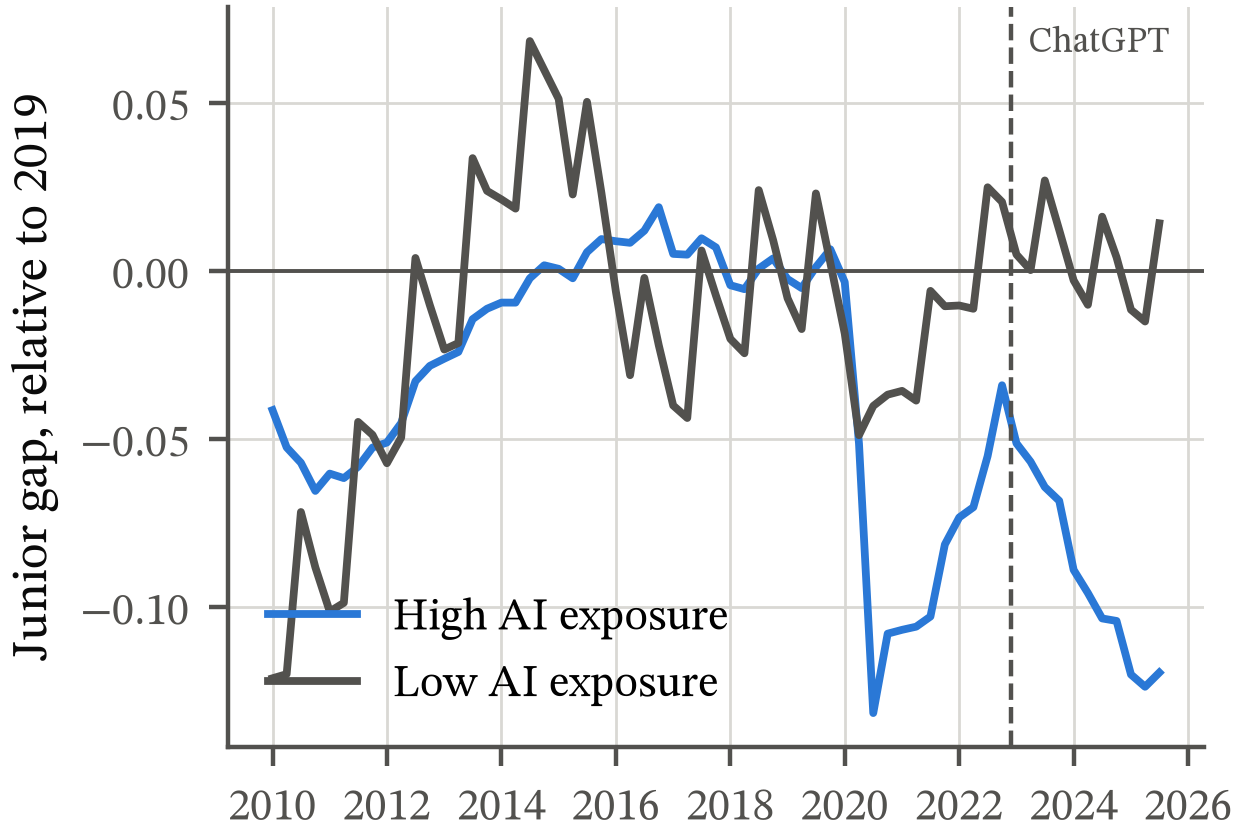
\includegraphics[width=\linewidth]{fig01_junior_gap_by_exposure.png}
    \caption{Junior employment gap}
    \label{fig:raw-junior}
  \end{subfigure}\hfill
  \begin{subfigure}[t]{0.49\textwidth}
    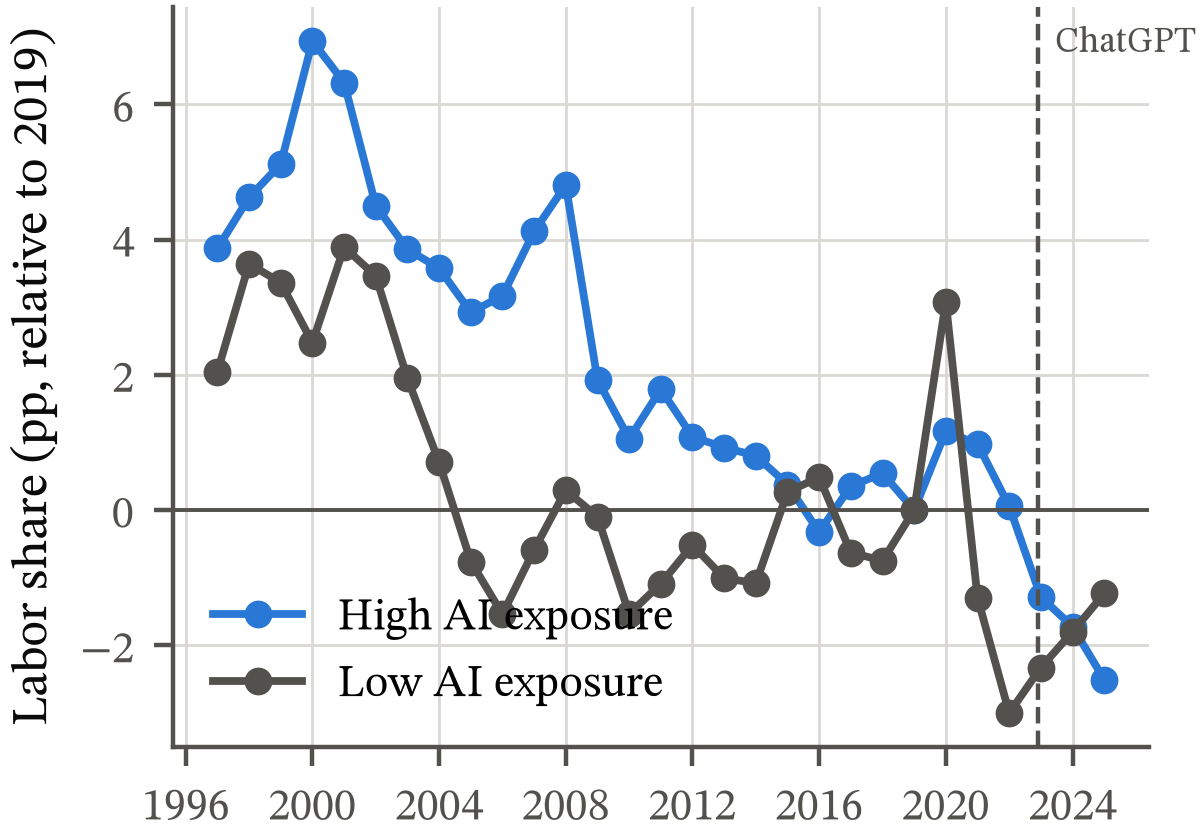
\includegraphics[width=\linewidth]{fig04_labor_share_by_exposure.png}
    \caption{Labor share of value added}
    \label{fig:raw-labor}
  \end{subfigure}
  \caption{Raw data. (a) Log employment of 22--24 year-olds minus log employment of 35--54 year-olds (Census QWI), averaged within the top and bottom thirds of sectors by language-model AI exposure, relative to 2019. (b) Compensation over value added (BEA), averaged within sectors above and below median AI exposure, relative to 2019. These are descriptive; Section~\ref{sec:results} controls for common shocks.}
  \label{fig:raw}
\end{figure}

Figure~\ref{fig:raw} shows the two raw facts that the rest of the paper tests. In high-exposure sectors the junior employment gap collapsed in 2020, recovered through 2022, and has fallen steadily since ChatGPT's release in November 2022; low-exposure sectors show no such pattern. The labor share of high-exposure sectors, which sat above that of low-exposure sectors for most of the last two decades, has fallen below it since 2023. Both pictures are descriptive. A common shock (the 2022--23 rate cycle, for instance) could produce either, and the high-exposure group is dominated by finance and information, whose margins respond to interest rates for reasons that have nothing to do with AI. The empirical design in Section~\ref{sec:data} exists to separate these stories.

\section{Economic Mechanism and Asset-Pricing Channel}
\label{sec:mechanism}

\paragraph{What we claim to forecast better than the market.} The market treats ``AI exposure'' as a single characteristic: high-exposure industries are expected to benefit. Model~\eqref{eq:tasks} says the same exposure can mean opposite things for shareholders. If AI replaces the routine (often junior) tasks in an industry, measured hours fall relative to output, unit labor costs fall, and the gain shows up in gross operating surplus. If AI complements the workers who remain, output rises but so do wages, and margins need not move. The labor-market data distinguish these cases months or years before they show up in earnings; equity prices may not.

\paragraph{Chain from macro information to prices.} The mechanism runs as follows.
\begin{enumerate}
  \item \emph{Firm reaction functions} (secondary channel): firms adopt AI for codified tasks and cut entry-level hiring before they cut existing staff, because attrition is cheaper than layoffs.
  \item This appears first in the employment-by-age data (QWI) and in the supervisory share of employment (CES), and only later in output and compensation by industry (BEA).
  \item \emph{Cash flows} (primary channel): lower unit labor costs raise margins in substituting industries; the labor share falls.
  \item If investors underweight these releases, prices of substituting industries drift up relative to complementing industries as the cash flows are realized.
\end{enumerate}
\emph{Discount rates} enter as a confound rather than a channel. AI-exposed sectors (information, finance, professional services) are long-duration and rate-sensitive, so any return pattern must survive a control for exposure to the 2-year Treasury yield (Lecture~7).

\paragraph{Four claims and what would refute them.} Every result in this paper maps to one of four claims, each with a stated falsifier.

\begin{singlespace}
\small
\begin{center}
\begin{tabular}{p{0.06\linewidth}p{0.42\linewidth}p{0.42\linewidth}}
\toprule
 & Claim & Inconsistent evidence \\
\midrule
C1 & Output per hour accelerated more where AI exposure is higher. & No exposure gradient, or one driven only by price-deflator artifacts in the information sector. \\
C2 & Substitution shows up as missing junior workers, adjusting through hiring rather than separations. & The same junior decline in low-exposure sectors (a common shock), or one explained by sector size (demand). \\
C3 & Substitution raises margins: the labor share falls where exposure is high. & Prices fall one-for-one with any productivity gain (gains go to consumers), or the result rests on one sector. \\
C4 & The market does not separate substituting from complementing sectors, so a long-short on the substitution signal earns alpha. & No alpha after factor controls, or returns explained by interest-rate exposure. \\
\bottomrule
\end{tabular}
\end{center}
\end{singlespace}

\paragraph{Why test twice.} With roughly three years of post-ChatGPT data, any AI-era estimate is noisy. The IT boom gives us a second, completed episode of a general-purpose technology hitting white-collar work. We estimate every claim on both episodes with identical code, using 1995 IT capital intensity as the IT-era analogue of AI exposure, and then ask how far the AI-era evidence should be pulled towards the IT-era estimate (Section~\ref{sec:bayes}). The two exposure measures are correlated (0.63 across sectors), so the same white-collar sectors are ``exposed'' in both eras; differences in outcomes are therefore informative about the technology rather than about which sectors we happen to be looking at.

\section{Data and Event Selection}
\label{sec:data}

All data are free and public. Table~\ref{tab:data} lists each source with its release frequency and publication lag; the code that downloads and transforms them is public (Appendix~\ref{app:code}).

\begin{table}[t]
\caption{Data sources. ``Lag'' is the approximate time between the end of the reference period and publication.}
\label{tab:data}
\begin{singlespace}\small\centering
\begin{tabular}{p{0.27\linewidth}p{0.33\linewidth}p{0.13\linewidth}p{0.15\linewidth}}
\toprule
Object & Source (release) & Frequency & Coverage, lag \\
\midrule
Real value added, compensation, prices by industry & BEA GDP by Industry & A (Q) & 1997 (2005)--2026Q2; $\sim$3 months \\
Employment, hours, supervisory share & BLS Employment Situation (CES), via FRED & M & 1964--Oct 2026; 1 month \\
Employment and hires by age $\times$ sector & Census QWI, national file & Q & 1994Q1--2025Q3; $\sim$12 months \\
Unemployment by age (20--24, 25--54) & BLS CPS, via FRED & M & 1948--Oct 2026; 1 month \\
AI exposure by industry & \citet{felten2023language}, language-model AIIE & static & NAICS 4--6 digit \\
IT capital by industry, 1995 & BEA detailed fixed assets & A & 1925--2025 \\
Industry returns, factors & Ken French data library & D & through Sep 2026 \\
2-year Treasury yield & FRED (DGS2) & D & through Nov 2026 \\
\bottomrule
\end{tabular}
\end{singlespace}
\end{table}

\paragraph{Units of analysis.} Output per hour (C1) and the labor share (C3) are measured for 13 private sectors where BEA's industry definitions match a CES supersector. Employment by age (C2) uses the 19 two-digit NAICS sectors in QWI. Total employment is measured for 91 detailed CES industries matched to the exposure index at the 3- or 4-digit NAICS level. Returns (C4) use 16 sectors formed by mapping the 49 Fama--French industries to NAICS sectors.

\paragraph{Key transformations.}
\begin{itemize}
  \item \emph{Hours.} CES publishes all-employee hours only from 2006, so for earlier years we scale the production-and-nonsupervisory hours index by the ratio of all to nonsupervisory employment, and splice it to the official series in 2006. The proxy tracks the official series within $\pm5\%$ over 2006--2026. Using nonsupervisory hours alone would overstate productivity in exactly the industries where AI removes nonsupervisory jobs.
  \item \emph{Junior gap.} $g_{s,t} = \ln E_{s,t}^{22\text{--}24} - \ln E_{s,t}^{35\text{--}54}$ from QWI; the analogous hiring gap uses QWI hires.
  \item \emph{Exposure.} AI exposure is the mean language-model exposure score across detailed industries in a sector; IT exposure is the IT (computers, communications, software) share of the sector's net capital stock in 1995. Both are standardized across sectors, so coefficients are per standard deviation.
\end{itemize}

\paragraph{Event windows and timing.} The AI era starts with ChatGPT's release (November 30, 2022). COVID quarters (2020--2021) are excluded from every estimate, because the hours and employment of exposed sectors collapsed and rebounded for unrelated reasons. For trading, a QWI quarter is treated as known only 12 months after it ends, matching the observed publication lag; BEA and CES data are used with their release lags.

\paragraph{Announced value versus market expectation.} These releases have no consensus forecasts, which is one reason we expect slow price responses. We form a ``prior'' for the slowest release instead: a nowcast of the QWI junior gap from monthly CES employment, the CES supervisory share and the CPS young-minus-prime unemployment gap, fitted on 2001--2019 only. Out of sample (2023--2025) it explains 53\% of the variation in the realized junior gap (correlation 0.77; Figure~\ref{fig:nowcast} in Appendix~\ref{app:nowcast}).

\paragraph{Limitations.} FRED and the bulk files serve the latest data vintage; revisions are not modeled except through the conservative QWI lag. National QWI aggregates include imputed values for early years. Exposure is averaged without employment weights. The Fama--French to NAICS mapping is approximate (for example, ``Business Services'' covers both NAICS 54 and 56).

\subsection{Empirical design}
\label{sec:design}

For each claim and era $e \in \{\text{IT}, \text{AI}\}$ we estimate
\begin{equation}
  y_{s,t} = \mu_s + \lambda_t + \beta_e \left(\text{Era}_t \times \text{Exposure}_s\right) + \gamma' x_{s,t} + \varepsilon_{s,t},
  \label{eq:did}
\end{equation}
where $\mu_s$ and $\lambda_t$ are sector and period fixed effects. The period effects absorb everything common to all sectors (the business cycle, monetary policy, the 2022--23 hikes), so $\beta_e$ is identified only from differences across sectors with different exposure. For C1 and C3 the IT era is 1998--2004 and the AI era 2023--2025, each compared with a common 2010--2019 baseline. For C2 the IT window is 1996--2000 against 1994--1995 and the AI window is 2022Q4--2025Q3 against 2015--2019; $x_{s,t}$ optionally includes log sector employment, so that the junior gap is measured \emph{given} sector size.

With 13 to 19 sectors, conventional clustered standard errors over-reject. We therefore report $p$-values from the restricted wild cluster bootstrap with Webb weights \citep{cameron2008bootstrap, webb2023reworking}, 1,999 replications. To check timing, we estimate year-by-year versions of~\eqref{eq:did} (event studies) and a ``kink'' specification that adds, interacted with exposure, a pre-existing trend, a post-COVID level shift, and a post-ChatGPT change in slope.

\section{Results}
\label{sec:results}

Table~\ref{tab:did} reports every estimate of~\eqref{eq:did}; Figure~\ref{fig:claims} plots the three headline coefficients side by side for the two eras. The short version: the AI era looks nothing like the IT boom in the labor data, and the difference points to substitution.

\begin{table}[t]
\caption{Difference-in-differences estimates of~\eqref{eq:did}. Each coefficient is the change in the outcome during the era, relative to baseline, for a sector one standard deviation more exposed. Standard errors are clustered by sector; $p_{\text{boot}}$ is from the wild cluster bootstrap (Webb weights, 1,999 replications). C1 and C3: 13 sectors, annual. C2: 19 sectors, quarterly.}
\label{tab:did}
\inserttable{tab_did}
\end{table}

\begin{figure}[t]
  \centering
  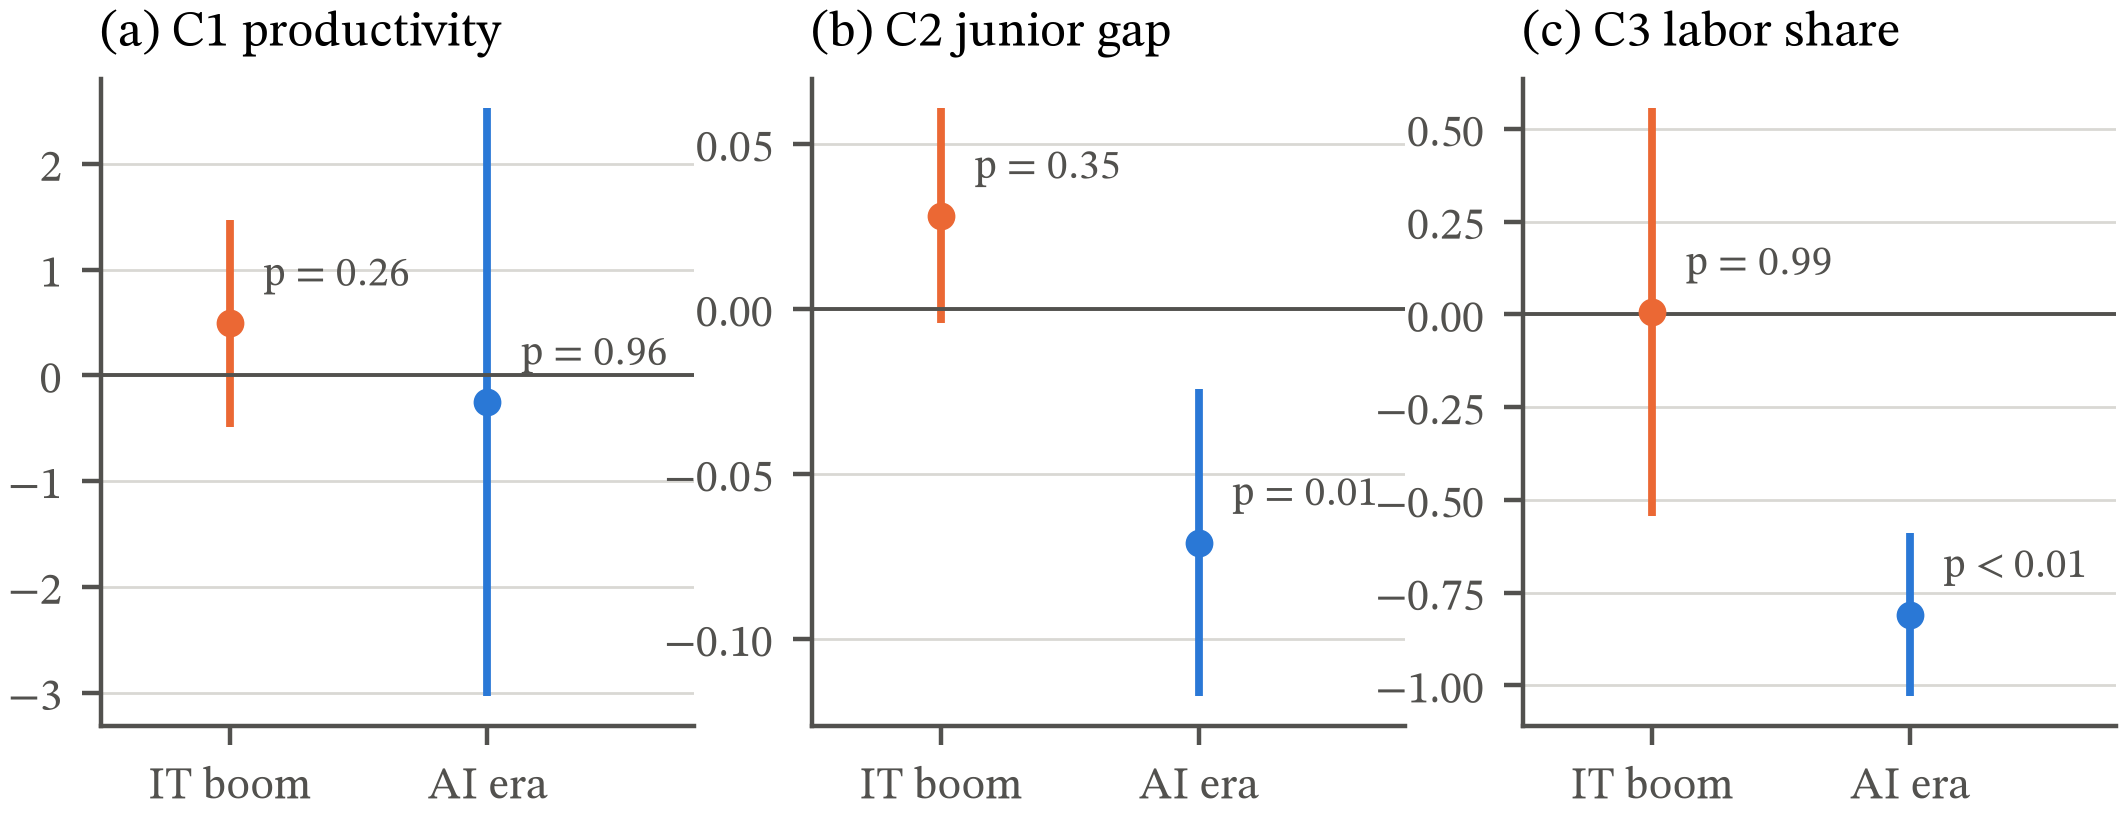
\includegraphics[width=\textwidth]{fig03_claims_it_vs_ai.png}
  \caption{IT boom versus AI era. Coefficients from Table~\ref{tab:did} with 95\% intervals and bootstrap $p$-values: (a) output per hour growth, pp per year; (b) junior employment gap given sector size, log points; (c) change in the labor share, pp per year. Orange: IT boom, exposure is the 1995 IT capital share. Blue: AI era, exposure is language-model AI exposure.}
  \label{fig:claims}
\end{figure}

\subsection{C1: no productivity acceleration yet}

Output per hour did not accelerate faster in AI-exposed sectors. The AI-era coefficient is $-0.26$ percentage points per year per standard deviation, with a standard error of 1.42 and a bootstrap $p$ of 0.96. In the IT boom the estimate is $+0.49$, positive as \citet{stiroh2002it} found but imprecise with 13 sectors ($p=0.26$). We read the AI-era null with care. It is a statement about measured output: when a firm buys an AI service, the purchase is an intermediate input and is subtracted from the firm's value added (Assignment~1, Question~1). A firm that uses AI to replace a junior analyst may produce the same output with fewer hours, which raises output per hour, or the same hours with a higher bill for purchased services, which does not. Measured productivity in the user industry then understates the gain, which is consistent with the J-curve argument of \citet{brynjolfsson2021jcurve}. Our earlier descriptive table, which suggested a white-collar productivity surge, did not survive the switch to all-employee hours and the inclusion of time effects; we discarded it.

\subsection{C2: the missing juniors}

The clearest result is in employment by age. In the AI era, a sector one standard deviation more exposed saw the employment of 22--24 year-olds fall by 4.9 log points relative to 35--54 year-olds in the same sector; holding sector size fixed the decline is 7.1 log points (bootstrap $p=0.01$). The hiring gap moves in the same direction ($-3.3$ and $-4.6$ log points), consistent with adjustment through hiring rather than separations, as \citet{brynjolfsson2025canaries} find in ADP microdata. In the IT boom the sign is reversed (+3.2 and +2.8 log points) though not significant: computers complemented young, computer-literate workers.

\begin{figure}[t]
  \centering
  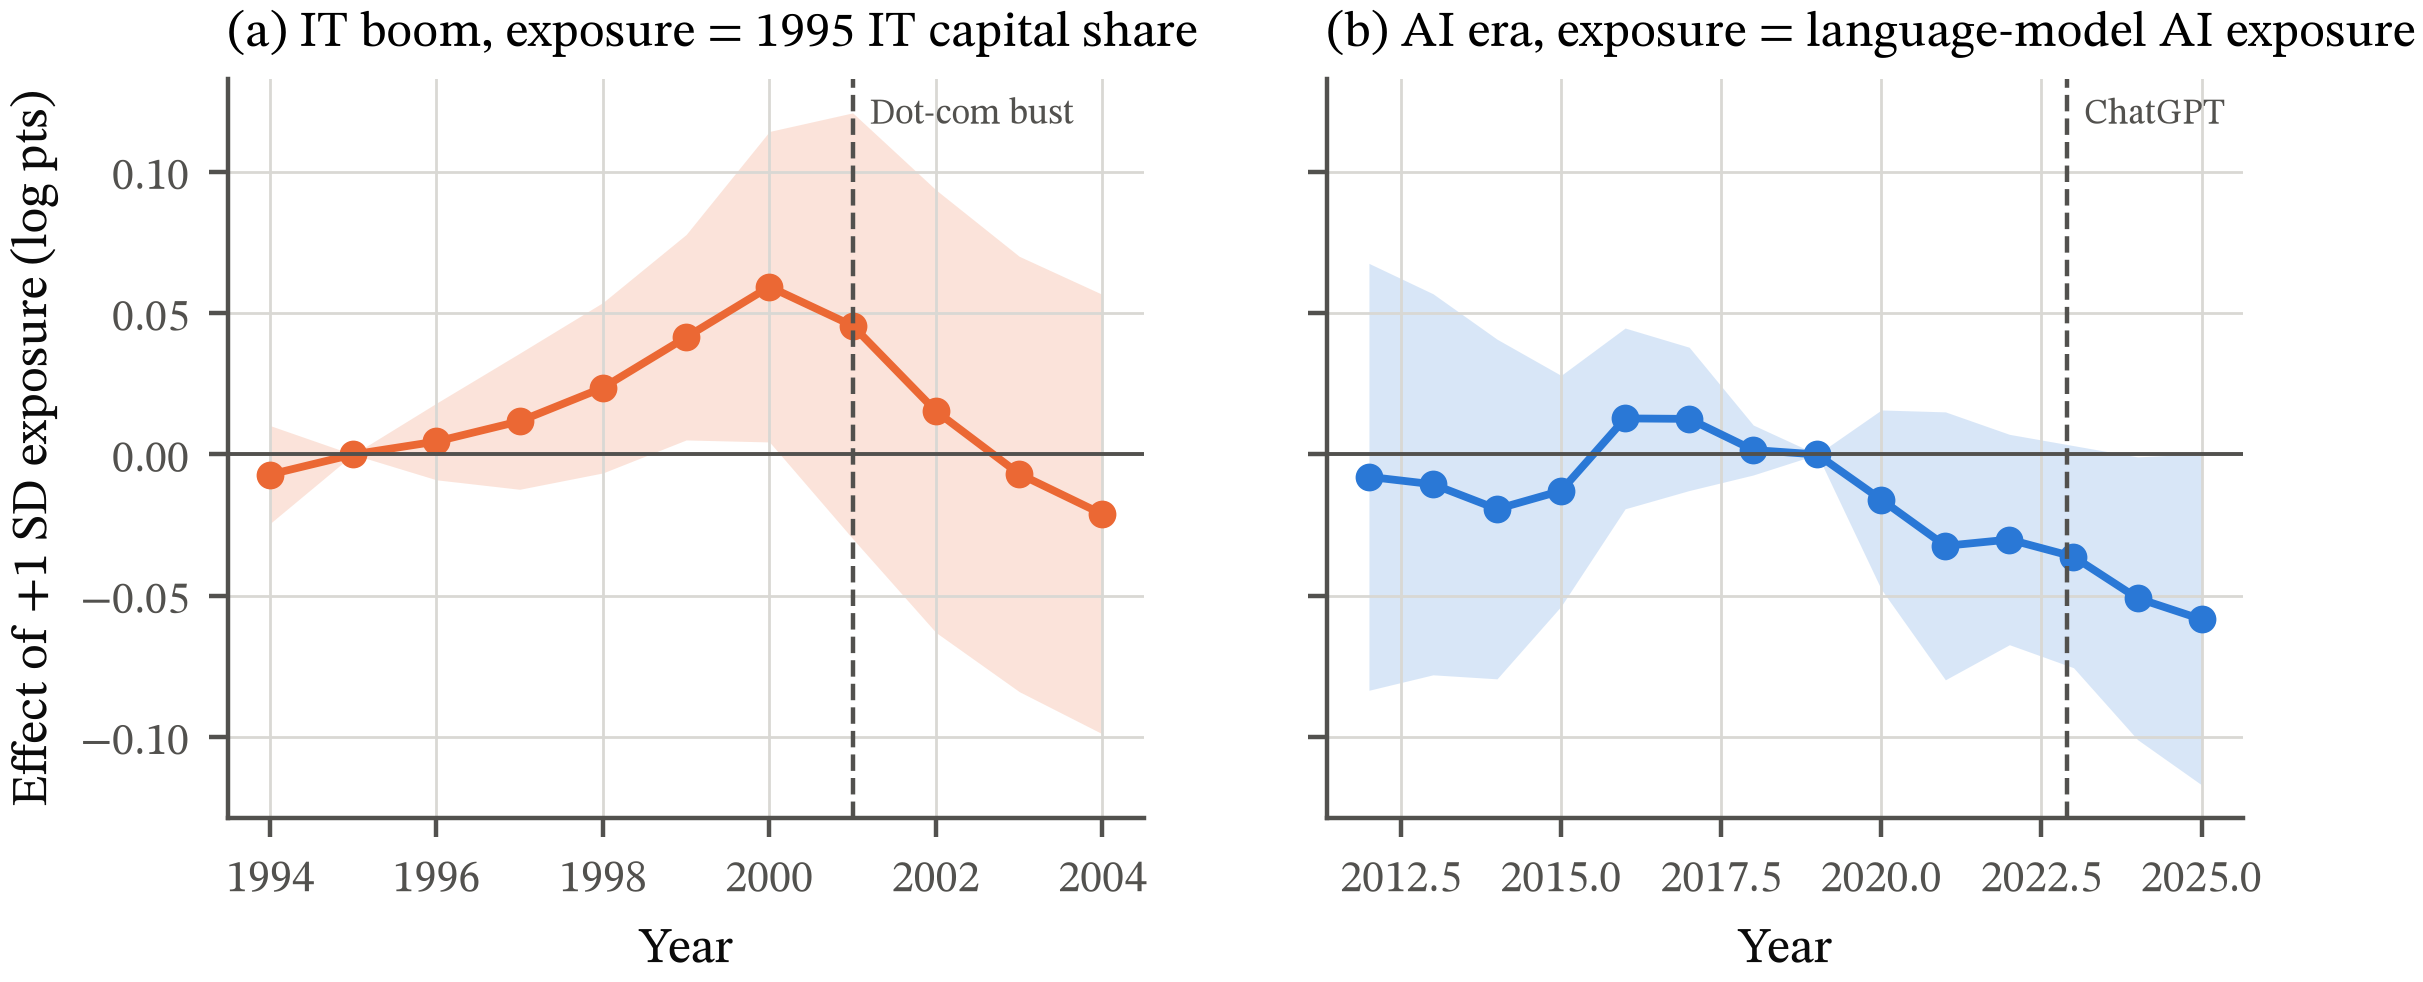
\includegraphics[width=\textwidth]{fig02_c2_event_studies.png}
  \caption{Event studies of the junior employment gap. Each point is the effect of one standard deviation of exposure on the junior gap in that year, relative to the base year (1995 for the IT boom, 2019 for the AI era), with 95\% intervals. (a) IT boom; the dashed line marks the 2001 dot-com bust. (b) AI era; the dashed line marks ChatGPT's release.}
  \label{fig:eventstudy}
\end{figure}

Timing matters for attribution, and Figure~\ref{fig:eventstudy} shows it. Panel (b) is flat from 2012 to 2019, so exposed sectors were not already shedding juniors. The decline starts in 2020, before ChatGPT, and continues through 2025. Panel (a) is a useful warning: in the IT boom, juniors in IT-intensive sectors gained through 2000 and lost those gains in the dot-com bust. Junior employment is cyclical; a hiring freeze in rate-sensitive sectors can look like technology.

\begin{table}[t]
\caption{Did the trend bend at ChatGPT? Each row is a term interacted with standardized AI exposure; COVID years (2020--2021) are dropped. The junior gap regression controls for sector size. Bootstrap $p$-values as in Table~\ref{tab:did}.}
\label{tab:kink}
\inserttable{tab_kink}
\end{table}

Table~\ref{tab:kink} separates the two stories. With COVID years dropped, exposed sectors show no pre-existing trend (0.0002 per year), a post-COVID level drop of 5.6 log points ($p<0.01$), and an \emph{additional} decline of 1.2 log points per year after ChatGPT ($p=0.01$). The level shift is consistent with remote work and the 2022 hiring freeze; the post-ChatGPT slope is what a substitution story predicts. This conclusion depends on how the COVID years are handled: an earlier specification that fitted a straight line through 2020--2022 averaged the crash and recovery into a single slope and found no post-ChatGPT kink. We report both, and treat the kink as suggestive rather than settled.

Total employment tells a different story from employment by age. Across 91 detailed CES industries, AI exposure predicts no change in total employment: no level shift, no kink (Table~\ref{tab:kink}, right columns; Figure~\ref{fig:detailed} in the appendix). AI is not, so far, reducing headcount in exposed industries; it is changing who is hired.

\subsection{C3: who gets paid}

The labor share answers the incidence question. In the AI era, a sector one standard deviation more exposed saw its labor share fall by 0.81 percentage points per year relative to baseline (bootstrap $p<0.01$); in the IT boom the estimate is zero (0.006, $p=0.99$). Because finance has by far the highest exposure, and its margins rose with interest rates in 2023--24 for reasons unrelated to AI, we re-estimate the model dropping one sector at a time. The coefficient stays between $-0.61$ (without finance) and $-0.85$, and every bootstrap $p$ stays below 0.01. Value-added prices in exposed sectors did not fall relative to others (+2.2 pp per year, $p=0.26$), so the gain was not passed on to consumers.

\subsection{Reading the three together}

The pieces fit one story. AI-exposed sectors are hiring fewer juniors, are not shrinking overall, are not (yet) producing measurably more per hour, and are paying a smaller share of their value added to labor. That is substitution at the entry margin, with the gain accruing to capital: the routine tasks of junior staff are being done by purchased AI services and by the seniors who remain. The IT boom, by contrast, looked like complementarity. For an investor this is a cash-flow signal (margins in exposed sectors should be higher than their measured productivity suggests), which brings us to whether prices reflect it.

\subsection{Pooling the IT prior with AI-era evidence}
\label{sec:bayes}

How much should the IT boom inform our reading of AI? We treat the IT-era estimate as a prior for the AI-era coefficient, $\beta_{AI} \sim N(\hat\beta_{IT}, \mathrm{se}_{IT}^2 + \tau^2)$, where $\tau$ measures how different we allow AI to be, and update with the AI-era estimate. Figure~\ref{fig:bayes} traces the posterior as $\tau$ widens. For C3 the AI data dominate even at $\tau=0$: the posterior mean is $-0.70$, because the AI-era estimate is far more precise than the prior. For C2 the conclusion depends on beliefs: if AI is assumed identical to IT the posterior is centered near zero, but once $\tau$ reaches the AI-era standard error the probability that the effect is negative rises to 0.95. For C1 neither era is informative.

\begin{figure}[t]
  \centering
  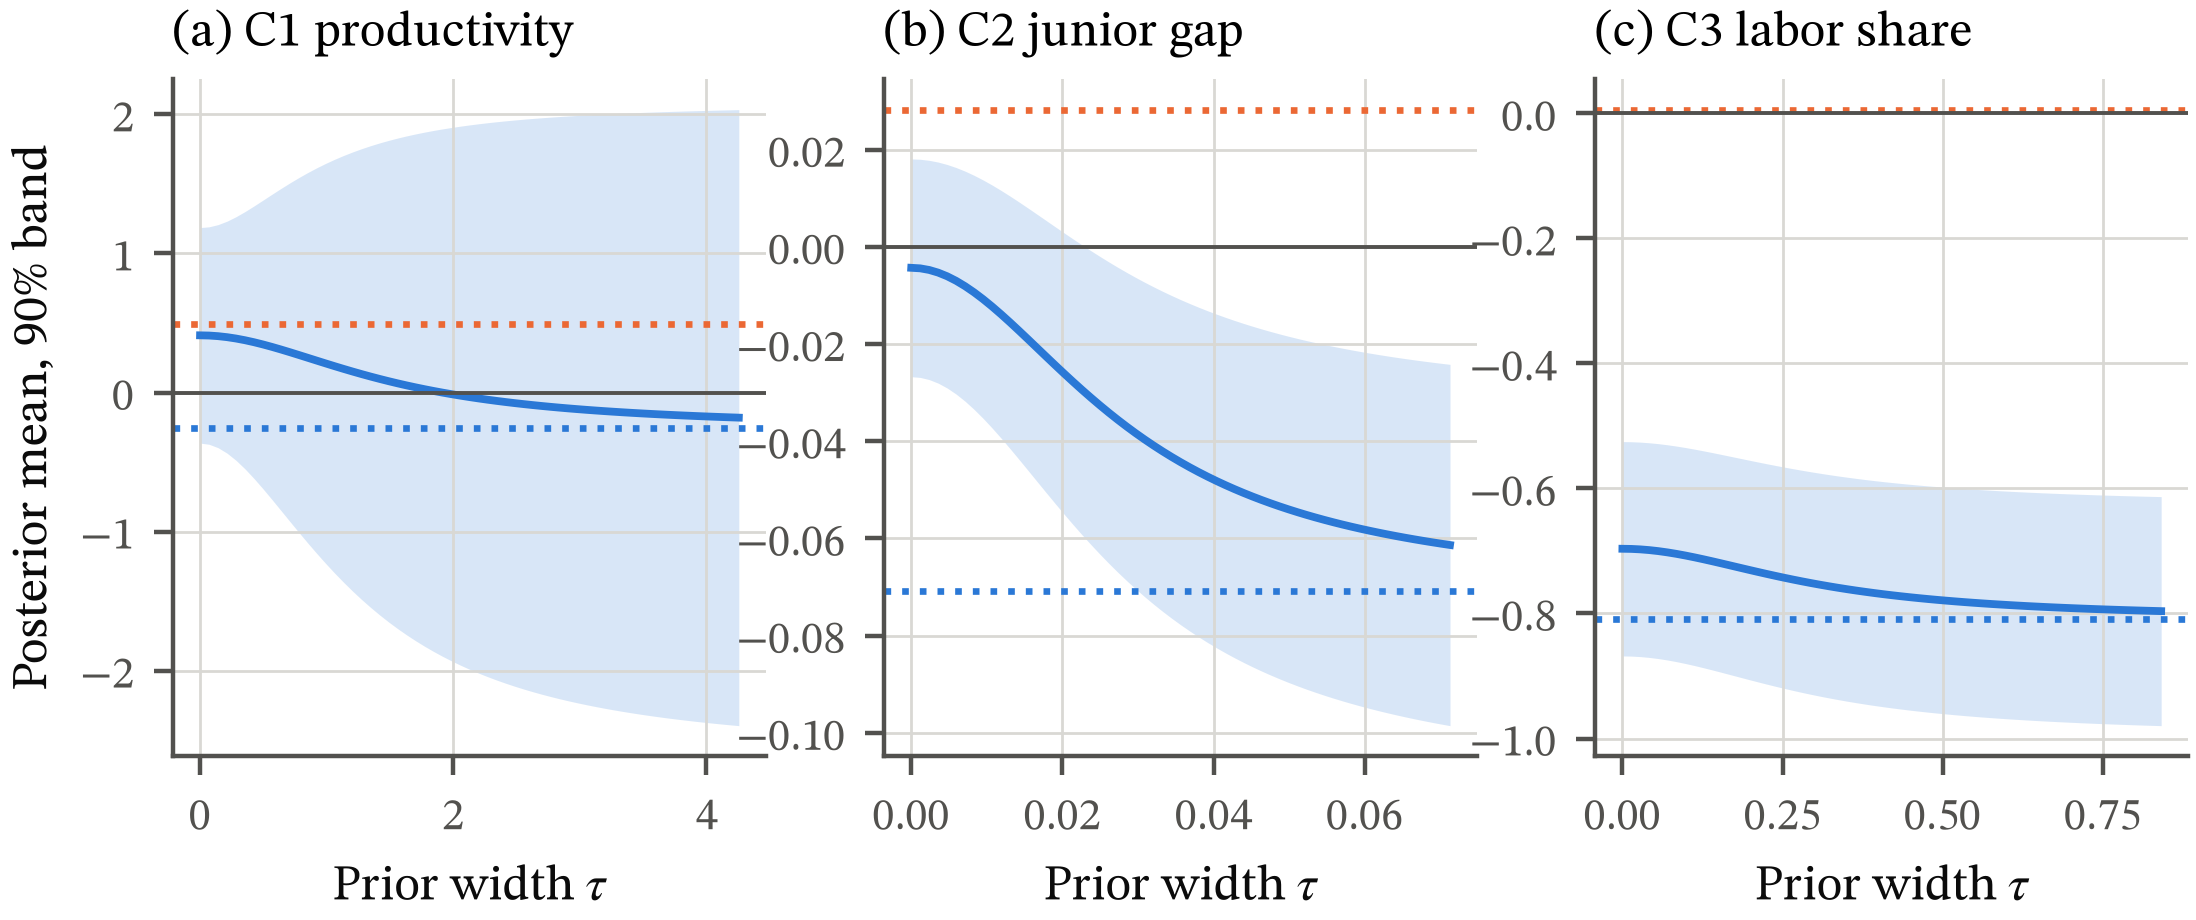
\includegraphics[width=\textwidth]{fig08_bayesian_pooling.png}
  \caption{Posterior of each AI-era coefficient when the IT-boom estimate is used as a prior, as the prior width $\tau$ increases from ``AI is exactly IT'' ($\tau=0$) to ``AI is new''. Solid line: posterior mean, with 90\% band. Dotted lines: the IT-era estimate (orange) and the AI-era estimate (blue).}
  \label{fig:bayes}
\end{figure}

\section{Forward-Looking Discussion}
\label{sec:forward}

Past behavior around the IT boom is a poor template for AI, and our results say exactly where. Table~\ref{tab:diffs} lists the differences we think matter and what each predicts in the data. The first two are already visible: the sign of the junior-employment effect flipped between eras. The third and fourth explain why measured productivity may lag. The fifth is the one that would most change the investment case.

\begin{table}[t]
\caption{How generative AI differs from the 1995--2004 IT boom, and where each difference should show up.}
\label{tab:diffs}
\begin{singlespace}\small\centering
\begin{tabular}{p{0.04\linewidth}p{0.38\linewidth}p{0.47\linewidth}}
\toprule
 & Difference & Prediction and status \\
\midrule
D1 & IT automated routine middle-skill tasks; AI targets codified cognitive tasks in white-collar work. & Knowledge work flips from complement to substitute. \emph{Seen:} C2 sign flip. \\
D2 & IT rewarded computer-literate graduates; AI substitutes for the entry-level tasks that juniors learn on. & Junior--senior gap opens only in the AI era. \emph{Seen:} C2 and the kink test. \\
D3 & IT required heavy user-side capital and reorganization; AI is rented per use. & Faster adoption, less capital deepening at users. \emph{Not yet tested.} \\
D4 & Purchased AI services are intermediate inputs; user value added rises only if output rises by more. & Measured user productivity understates gains. \emph{Consistent with} C1 null and C3. \\
D5 & IT hardware was competitive; AI supply (chips, frontier models) is concentrated. & Producers may capture the gain through pricing, shrinking user margins over time. \emph{Watch:} intermediate-input costs in exposed sectors. \\
D6 & The Fed let 1990s productivity growth run; 2022--26 is a hiking cycle, with a further hike in September 2026. & Hiring freezes in rate-sensitive sectors mimic substitution; discount-rate effects dominate returns. \emph{Seen:} C4 rate loading. \\
\bottomrule
\end{tabular}
\end{singlespace}
\end{table}

\paragraph{Current conditions.} The FOMC raised the federal funds target to 3.75--4\% in September 2026 with inflation above target. Two consequences follow for this trade. First, rate-sensitive sectors are also the AI-exposed ones, so any long-short on exposure carries duration risk; our strategy's returns after ChatGPT load positively on the 2-year yield ($t=2.6$, Table~\ref{tab:strategy}). Second, tight policy is itself a reason for firms to freeze junior hiring, which makes the labor signal harder to read in real time. Our nowcast suggests the junior gap kept widening through 2026, by about 1.7 log points over the year to 2026Q3.

\paragraph{What would change our view.} Three developments would make the trade more attractive: (i) a measurable productivity acceleration in exposed user industries, which would confirm that the margin gains are durable; (ii) evidence that AI vendors are \emph{not} capturing the surplus (falling per-unit AI prices that do not raise user input costs); and (iii) an easing cycle, which would reduce the rate component of sector returns. A reversal of the junior decline as the 2026 graduating class is absorbed would weaken the substitution reading altogether.

\paragraph{The bubble question.} The IT boom delivered real productivity gains and a crash in the stocks of the firms that sold the technology. Our evidence suggests a version of the same split: the economic gain from AI so far appears in the margins of the industries that \emph{use} it, while equity attention sits with the firms that \emph{sell} it. An investor worried about an AI valuation bubble in producers can hold the users whose labor data show substitution as a partial hedge; the hedge has economic logic even though, as the next section shows, it has not earned excess returns on its own.

\section{Trading Strategy Design and Performance}
\label{sec:strategy}

\paragraph{Signal.} For each sector, the substitution score is minus the four-quarter change in the QWI junior employment gap; a high score means juniors are losing ground fastest. A quarter's score is used only 12 months after the quarter ends, matching QWI's publication lag. A faster version would use the monthly nowcast (Section~\ref{sec:data}); we report the slow version because it uses only data that were public at the time.

\paragraph{Portfolio.} At the end of each month we rank the 16 sectors on the score and set dollar-neutral rank weights, $w_{s} \propto \operatorname{rank}(\text{score}_s) - \tfrac{N+1}{2}$, scaled to \$1 long and \$1 short, as in \citet{asness2013value}. Rank weights are insensitive to outliers. Weights are held for one month.

\paragraph{Sizing with a weak prior.} We do not know ex ante whether substituting sectors should outperform, so the sign is learned. Each month we update a normal posterior for the strategy's mean return, starting from a prior centered at zero, using only past returns with a five-year half-life (so that a regime change can overturn old evidence). The position is the posterior $z$-score of the mean, clipped to $[-1, 1]$. The strategy can therefore flip from long to short substituting sectors without any look-ahead.

\paragraph{Benchmark and controls.} We compare with a static long-short on AI exposure, the way the market is commonly assumed to trade AI. Each strategy is regressed on the Fama--French five factors \citep{fama2015five}, momentum \citep{carhart1997persistence}, and monthly changes in the 2-year Treasury yield, with Newey--West errors.

\begin{table}[t]
\caption{Backtest, January 1996 to September 2026, monthly. Mean, volatility and alpha are annualized; alpha is the intercept from a regression on the five Fama--French factors, momentum, and the monthly change in the 2-year Treasury yield ($\beta_{2y}$, return per percentage point), with Newey--West $t$-statistics.}
\label{tab:strategy}
\inserttable{tab_strategy}
\end{table}

\begin{figure}[t]
  \centering
  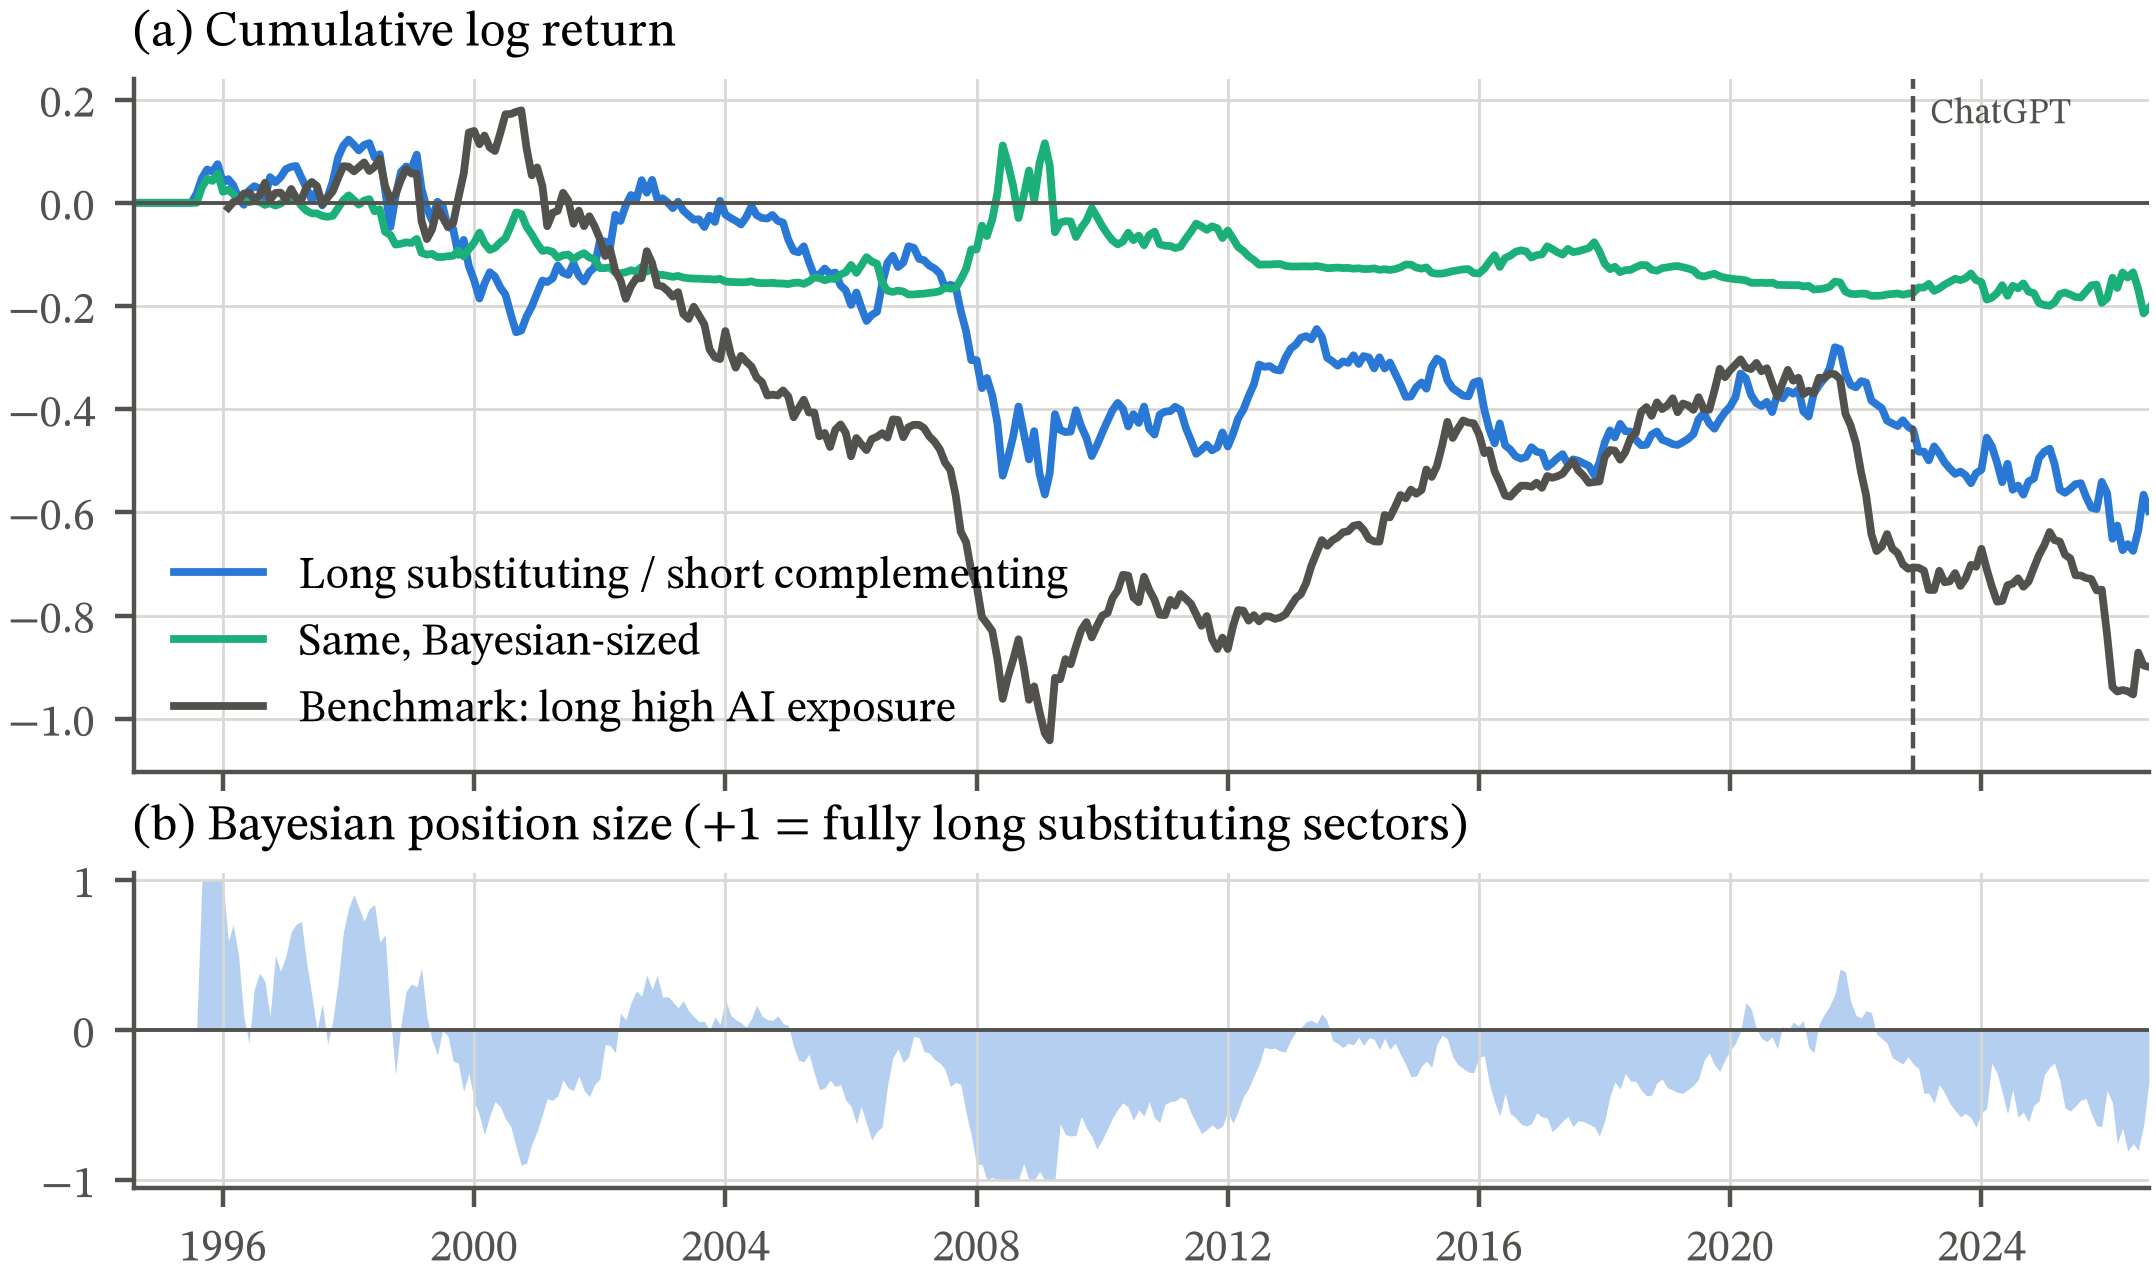
\includegraphics[width=\textwidth]{fig07_strategy.png}
  \caption{(a) Cumulative log returns of the substitution signal, the same signal with Bayesian sizing, and the AI-exposure benchmark. (b) The Bayesian position: $+1$ is fully long substituting sectors, $-1$ fully short.}
  \label{fig:strategy}
\end{figure}

\paragraph{Results.} Table~\ref{tab:strategy} and Figure~\ref{fig:strategy} report the backtest. The substitution signal loses 1.8\% a year with a Sharpe ratio of $-0.19$; its factor-adjusted alpha ($-1.6\%$, $t=-1.0$) is indistinguishable from zero. After ChatGPT the loss widens to 3.6\% a year and the returns load positively on the 2-year yield ($t=2.6$): the long side (substituting sectors) did better when rates rose, which is the discount-rate confound we expected. The Bayesian overlay learns to lean the other way for most of the period after 2000, which cuts volatility to 5.6\% and limits the drawdown to 28\%, but it earns nothing either. The AI-exposure benchmark is worse: $-2.5\%$ a year with a 71\% maximum drawdown, driven by 2008 and by 2022.

\paragraph{Why the result is negative, and why we stand by the analysis.} Three explanations fit the evidence. First, there may be no cash-flow signal to price yet: Section~\ref{sec:results} finds no clear change in the labor share of exposed sectors once the COVID spike is accounted for; and where margins do move, analysts see them quarterly in earnings, well before our 12-month-lagged QWI signal arrives. Second, sector returns are dominated by rate exposure in exactly the sectors we care about; with policy rates moving several hundred basis points in 2022--26, a cash-flow effect of a few percent a year is hard to detect in 16 portfolios. Third, the signal is noisy: turnover is about 127\% a year because quarterly changes in the junior gap are volatile. None of these says the real-side results are wrong. They say the real-side results are not, at sector level and with a one-year lag, a trading edge.

\paragraph{Implementation and risk.} If deployed, we would trade sector ETFs, hedge the 2-year rate exposure with Treasury futures sized by each sector's trailing rate beta, smooth the signal over eight quarters to cut turnover, and use the monthly nowcast to reduce the lag. Position limits and the Bayesian sizing cap drawdowns; the main residual risk is a regime change in rate policy that moves exposed sectors together.

\section{Conclusion}
\label{sec:conclusion}

AI is showing up in the macro data, but not where the productivity narrative expects. Measured output per hour in exposed sectors has not accelerated, and total employment in exposed industries has not changed. What has changed is the composition of hiring: exposed sectors employ markedly fewer young workers relative to prime-age workers, a pattern that began with COVID and, in our preferred specification, steepened after ChatGPT. The 1995--2004 IT boom shows the opposite sign, which is itself evidence that AI is a different kind of technology for white-collar work. Whether the gain is reaching shareholders is not yet visible; the labor share of exposed sectors has returned to about its 2019 level after a COVID-era spike.

For an investor, the result is an early labor-market signal that has not yet become a cash-flow signal, and that is drowned out by rate exposure at sector level. A long-short strategy on the junior-substitution signal did not earn excess returns from 1996 to 2026. We would not deploy it as a stand-alone strategy. We would use the signal in two ways: as a filter when choosing among AI-exposed equities, and as an early warning. A clear fall in the labor share of exposed sectors over 2026--27 would turn the signal into a cash-flow story worth trading; a reversal of the junior decline would argue that the 2022--25 pattern was cyclical after all.

Four extensions would sharpen the analysis: event windows around BEA and QWI release dates using daily returns; employment-weighted exposure; firm-level labor and margin data, which would replace 16 sector portfolios with hundreds of stocks; and a markup measure that separates pricing power from substitution in the labor share.


\begin{singlespace}
\bibliographystyle{plainnat}
\bibliography{references}
\end{singlespace}

\appendix
\section{Technical Appendix}
\label{app:technical}

\subsection{Code and reproduction}
\label{app:code}

The pipeline is a Python package (\texttt{aiprod}) in the project repository,
\begin{center}\url{https://github.com/samaypanwar/ai-substitute-or-complement}.\end{center}
The single command \texttt{python -m aiprod.run} downloads every source, builds the panels, estimates all models, and writes the figures and the tables included in this paper; no number in a table is entered by hand.

\subsection{Wild cluster bootstrap}

For a coefficient $\beta_k$ we fit the model with $\beta_k=0$ imposed, keep its fitted values $\tilde y$ and residuals $\tilde u$, and draw for each sector $g$ a weight $v_g$ from Webb's six-point distribution $\{\pm\sqrt{3/2}, \pm1, \pm\sqrt{1/2}\}$. Each bootstrap sample is $y^* = \tilde y + v_g \tilde u$; we refit the full model and record the cluster-robust $t$-statistic for $\beta_k$. The $p$-value is the share of 1,999 bootstrap $|t^*|$ at least as large as the observed $|t|$.

\subsection{Bayesian pooling}

With prior $\beta_{AI} \sim N(\hat\beta_{IT}, \mathrm{se}_{IT}^2+\tau^2)$ and likelihood $\hat\beta_{AI} \sim N(\beta_{AI}, \mathrm{se}_{AI}^2)$, the posterior mean is $w\hat\beta_{AI} + (1-w)\hat\beta_{IT}$ with $w = (\mathrm{se}_{IT}^2+\tau^2)/(\mathrm{se}_{IT}^2+\tau^2+\mathrm{se}_{AI}^2)$.

\subsection{Nowcast of the junior gap}
\label{app:nowcast}

The nowcast regresses the four-quarter change in each sector's QWI junior gap on sector fixed effects and the four-quarter changes in log sector employment (CES), the supervisory share of employment (CES), and the young-minus-prime unemployment gap (CPS ages 20--24 minus 25--54). It is fitted on 2001--2019 and evaluated on 2023Q1--2025Q3.

\begin{figure}[h]
  \centering
  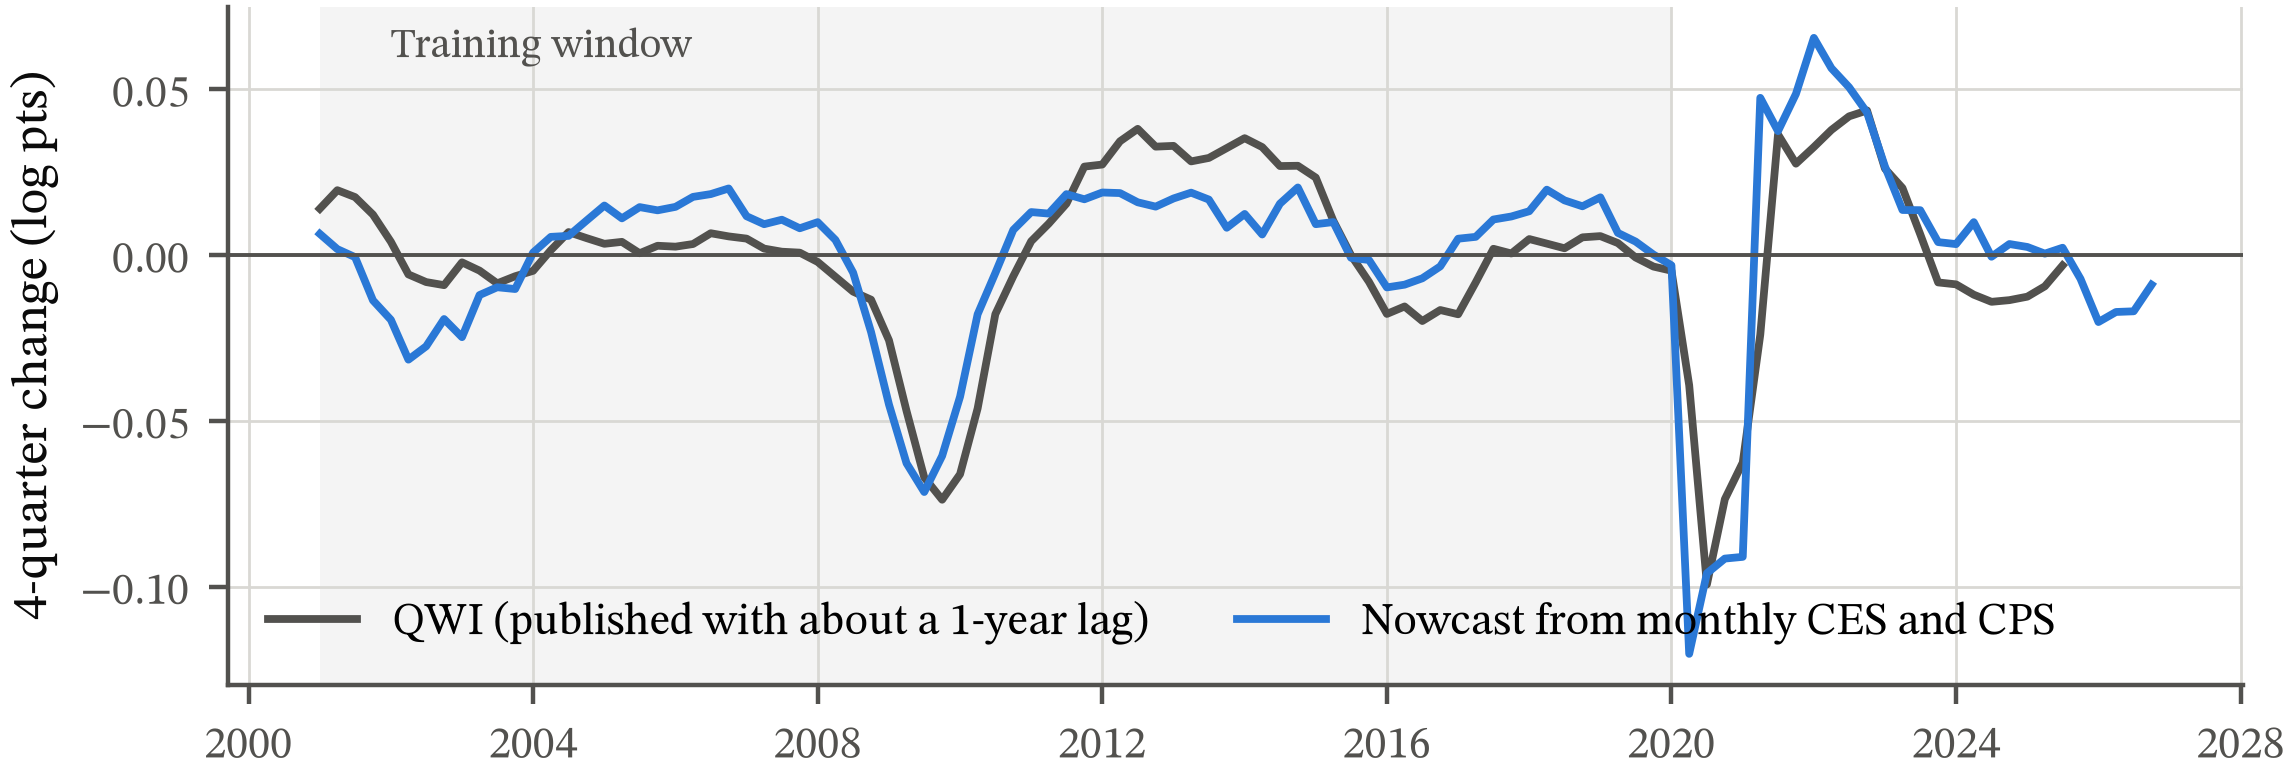
\includegraphics[width=\textwidth]{fig06_nowcast.png}
  \caption{Average four-quarter change in the junior employment gap across sectors: QWI as published (grey) and the nowcast from monthly data (blue). The shaded region is the training window; everything after 2019 is out of sample.}
  \label{fig:nowcast}
\end{figure}

\subsection{Additional figures}

\begin{figure}[h]
  \centering
  \begin{subfigure}[t]{0.49\textwidth}
    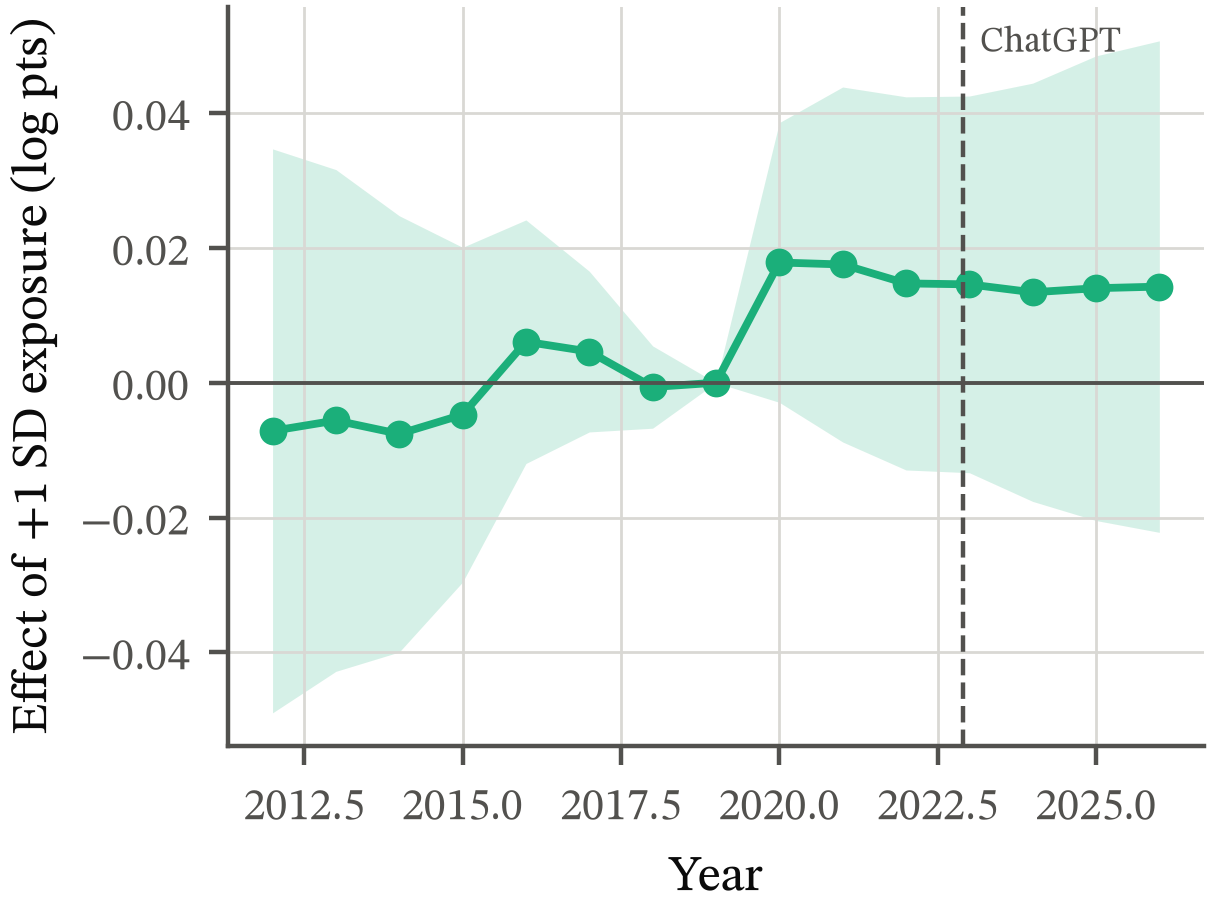
\includegraphics[width=\linewidth]{fig05_detailed_employment_event_study.png}
    \caption{Total employment, 91 detailed industries}
    \label{fig:detailed}
  \end{subfigure}\hfill
  \begin{subfigure}[t]{0.49\textwidth}
    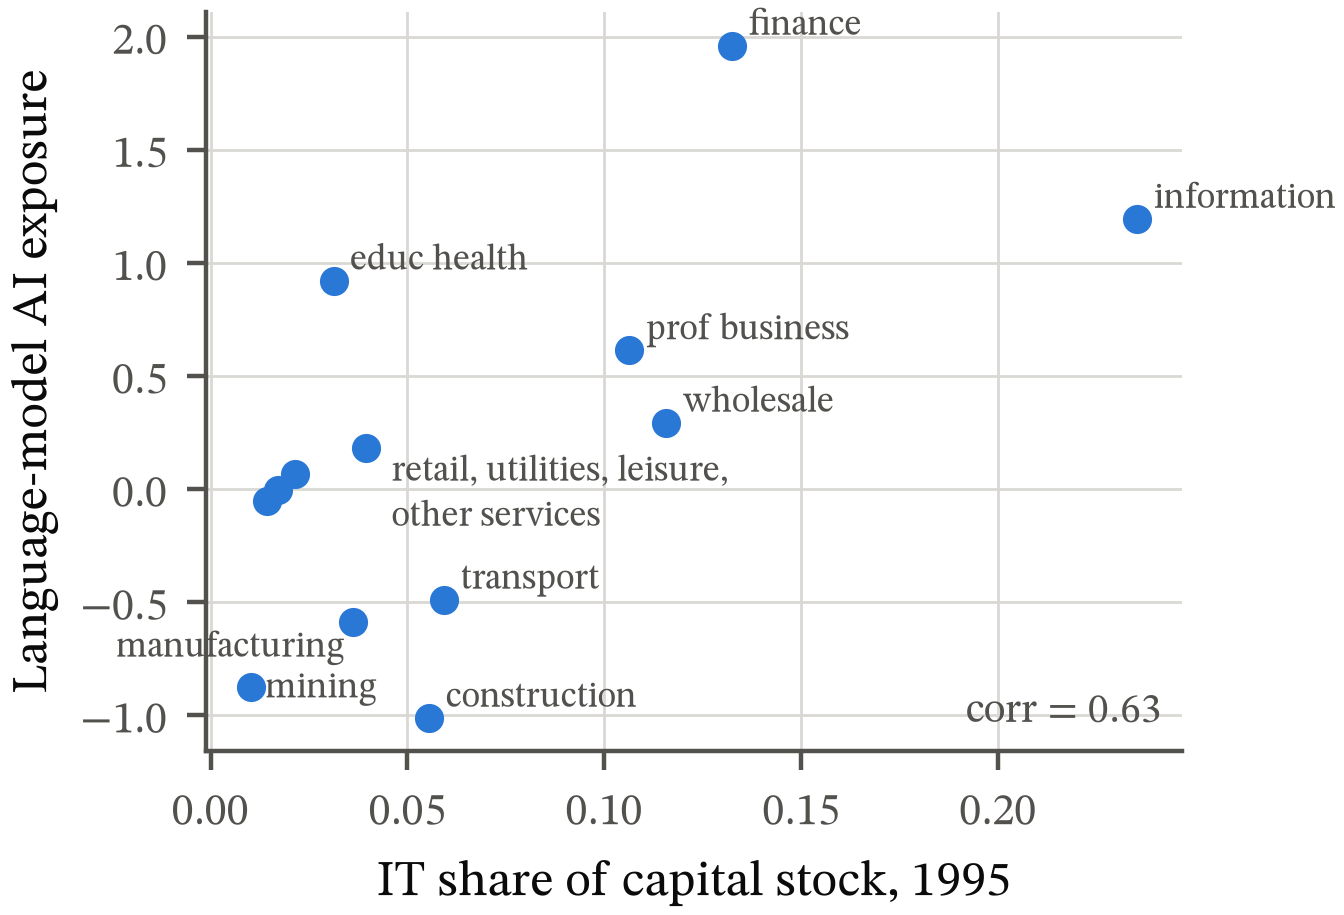
\includegraphics[width=\linewidth]{fig09_exposure_overlap.png}
    \caption{IT exposure versus AI exposure}
    \label{fig:overlap}
  \end{subfigure}
  \caption{(a) Event study of log total employment on AI exposure across 91 detailed CES industries, relative to 2019, with 95\% intervals; flat throughout. (b) Sector IT capital share in 1995 against language-model AI exposure (correlation 0.63).}
\end{figure}


\end{document}
